\section{Representación}

Dentro del contexto del UTRP, se pretende determinar un conjunto de rutas a partir de distintos paraderos de buses preestablecidos, los cuales deben presentar un beneficio para los pasajeros y para el operador del bus.\\

Para las paradas se utiliza un grafo no dirigido, cuyos vértices corresponden a las paradas y los arcos a un camino entre las paradas. Un ejemplo de esta representación es la red de Mandl, que puede apreciarse en la Figura \ref{fig:mandl}.

\begin{figure}[!htb]
\begin{center}
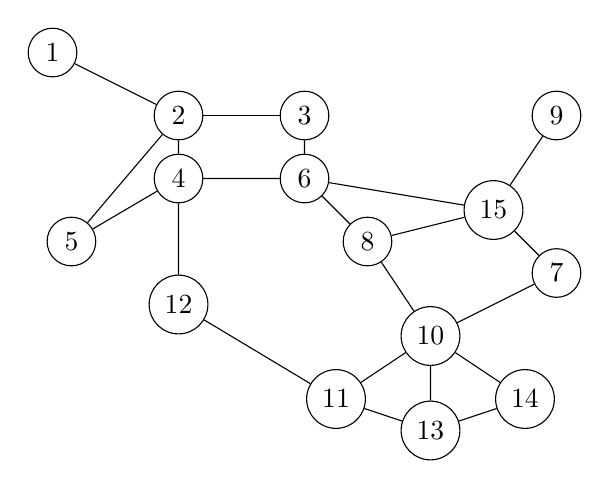
\begin{tikzpicture}[scale=0.8]
\node[draw,circle](1) at (0,0) { 1};
\node[draw,circle](2) at (2,-1) { 2};
\node[draw,circle](3) at (4,-1) { 3};
\node[draw,circle](4) at (2,-2) { 4};
\node[draw,circle](5) at (0.3,-3) { 5};
\node[draw,circle](6) at (4,-2) { 6};
\node[draw,circle](7) at (8,-3.5) { 7};
\node[draw,circle](8) at (5,-3) { 8};
\node[draw,circle](9) at (8,-1) { 9};
\node[draw,circle](10) at (6,-4.5) {10};
\node[draw,circle](11) at (4.5,-5.5) {11};
\node[draw,circle](12) at (2,-4) {12};
\node[draw,circle](13) at (6,-6) {13};
\node[draw,circle](14) at (7.5,-5.5) {14};
\node[draw,circle](15) at (7,-2.5) {15};

\draw (1) -- (2);
\draw (2) -- (3);
\draw (2) -- (4);
\draw (2) -- (5);
\draw (3) -- (6);
\draw (4) -- (5);
\draw (4) -- (6);
\draw (4) -- (12);
\draw (6) -- (8);
\draw (6) -- (15);
\draw (7) -- (15);
\draw (7) -- (10);
\draw (8) -- (10);
\draw (8) -- (15);
\draw (9) -- (15);
\draw (10) -- (11);
\draw (10) -- (13);
\draw (10) -- (14);
\draw (11) -- (12);
\draw (11) -- (13);
\draw (13) -- (14);
\end{tikzpicture}
\caption{Red de Mandl}
\label{fig:mandl}
\end{center}
\end{figure}

La representación utilizada en \cite{metaheuristic2010} para manejar el conjunto de rutas consiste en un arreglo bi-dimensional de $r$ filas y $m+1$ columnas, con $r$ la cantidad de rutas de la solución y $m$ la máxima cantidad de paraderos permitida. Cada fila distinta será una ruta, donde la primera columna almacena el número de la ruta. Para las otras columnas de la fila se utlizan identificadores para los paraderos de buses que componen la ruta. Por otra parte, los paraderos se encuentran representados por una matriz de demandas, una matriz de tiempos de viaje y por un sistema de coordenadas (este último para modelar la posición de cada paradero).

\begin{figure}[!htb]
\begin{subfigure}[b]{0.6\textwidth}
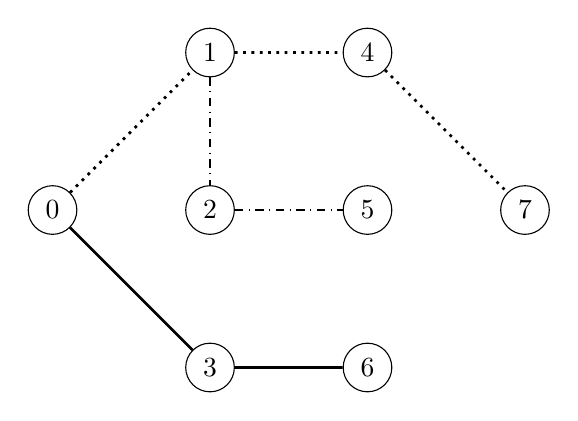
\begin{tikzpicture}
\node[draw,circle] (0) at (0,0) {$0$};
\node[draw,circle] (1) at (2,2) {$1$};
\node[draw,circle] (2) at (2,0) {$2$};
\node[draw,circle] (3) at (2,-2) {$3$};
\node[draw,circle] (4) at (4,2) {$4$};
\node[draw,circle] (5) at (4,0) {$5$};
\node[draw,circle] (6) at (4,-2) {$6$};
\node[draw,circle] (7) at (6,0) {$7$};

\draw[dotted, line width=1pt] (0) -- (1) -- (4) -- (7);
\draw[dash dot, line width=1pt] (1) -- (2) -- (5);
\draw[-, line width=1pt] (0) -- (3) -- (6);
\end{tikzpicture}
\caption{Grafo con tres rutas.}
\label{fig:grafo}
\end{subfigure}
\begin{subfigure}[b]{0.4\textwidth}
\begin{tabular}{|p{0.8cm}|p{0.8cm}|p{0.8cm}|p{0.8cm}|p{0.8cm}|}
\hline
R1 & 0 & 1 & 4 & 7\\
\hline
R2 & 0 & 3 & 6 & $*$\\
\hline
R3 & 1 & 2 & 5 & $*$\\
\hline
\end{tabular}
\caption{Arreglo bi-dimensional con tres rutas.}
\label{fig:tabla}
\end{subfigure}
\caption{Representación para el conjunto de rutas.}
\label{fig:repr1}
\end{figure}

Las matrices de tiempos de viaje y de demandas se representan mediante arreglos bidimensionales, donde la fila $i$ y columna $j$ aporta información entre el paradero $i$ y el paradero $j$.

Un ejemplo representación, considerando un grafo de 7 paraderos y 3 rutas distintas, están dadas la estructura de la Figura \ref{fig:repr1}. Se puede observar que la cantidad máxima de paraderos es 4, entonces la representación consiste de un arreglo de 3 filas y 5 columnas. El caracter asterisco al final de las rutas 2 y 3 denota que no hay un identificador de paradero, y por ende, la ruta tiene menos de cuatro paraderos.
